\chapter{Introduction}
The study of analyzing human movement traces its origins back to the 19th century, notably with Charles Darwin's investigations into the connection between movement and its meaning \cite{darwin}. 
Over the years, the fields of movement analysis and non-verbal communication have made significant progress in deciphering the significance of various movements. 
They have grappled with questions like, “Do movements convey meaning in their own right?" and “How do movements convey meaning?".\\
Movements and non-verbal expressions hold a unique place in communication as they transcend verbal language.
They contribute to the intricate web of conscious and subconscious communication during interactions \cite{Daly:1988, laffaye:2013}.

However, while there is a wealth of research exploring how emotions are conveyed through facial expressions and vocal cues, the role of full-body movement and expressive gestures in this context has been somewhat overlooked until recent times.

The need for further investigation arises from the rapid advancements in technology that have made full-body real-time movement analysis more accessible and affordable. 
Humans are adept at interpreting the emotional content of non-verbal cues, which underscores the importance of studying the perception of human motion \cite{samadani:2011}. 
Emotions have been observed to manifest through posture and movements, reinforcing the idea that movement plays a crucial role in how we perceive, understand and comunicate emotions in a nonverbal way \cite{gelder:2009,kleinsmith:2013,karg:2013}.

For example, the behaviour behind a “caress” can vary from care to hostility, 
if the origin of that movement is either the wrist, the shoulder or if it involves a complex contraction of muscle torques from the arm down to the leg. 
Nonetheless, the challenge lies in determining the correct interpretation of a specific movement.

\section{Origins and technological rise of Motion Capture}
The origin of motion capture can be traced back to the mid-20th century when rudimentary methods were employed, 
often involving manual tracking of key points on a subject's body. 
The introduction of marker-based MoCap in the 1970s marked a significant advancement. 
This technique involved attaching reflective markers to specific body points, which were then tracked by cameras to reconstruct the subject's movement in a digital environment. 
The example depicted in Figure \ref{fig:mocap_scene} illustrates two performers at the top engaged in a ball game, throwing it from one side to the other. Below, you can see the corresponding digital reconstruction. 
Technically, only the markers are automatically recognized, while the connections between markers are manually made, so these are later added.
\begin{figure}[H]
    \centering
    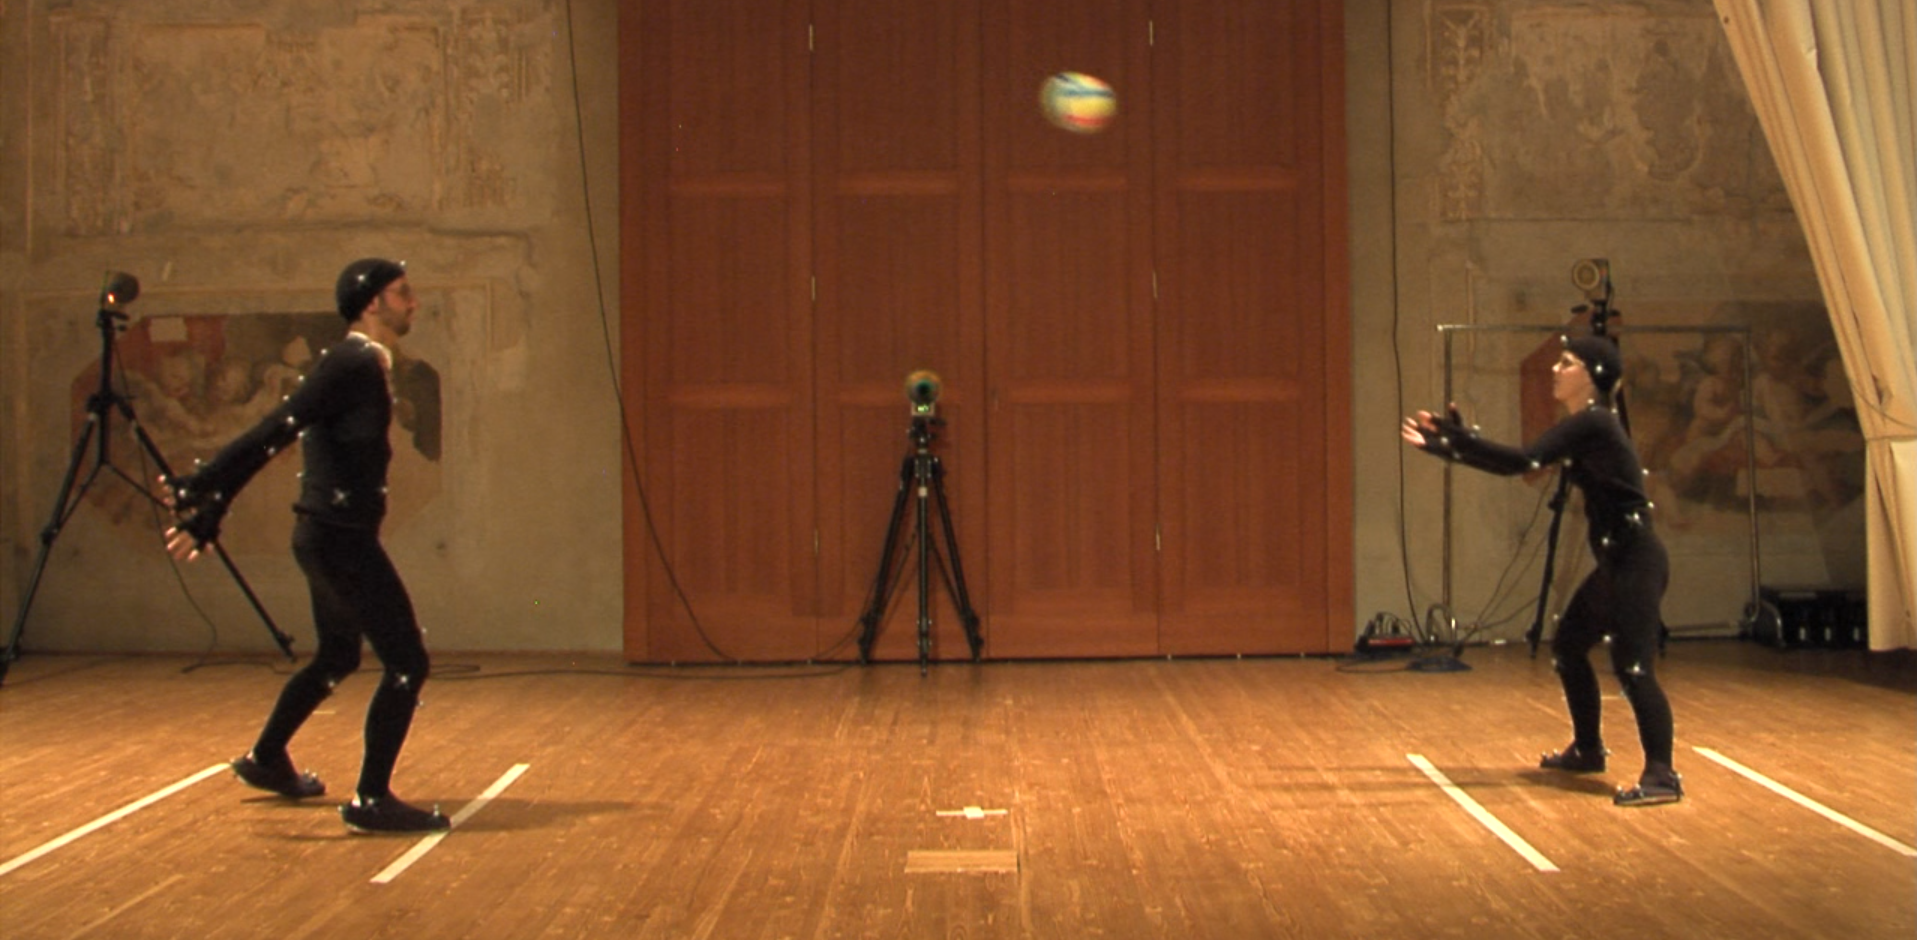
\includegraphics[width=0.75\textwidth]{bodyMarkersExampleImage.png}
    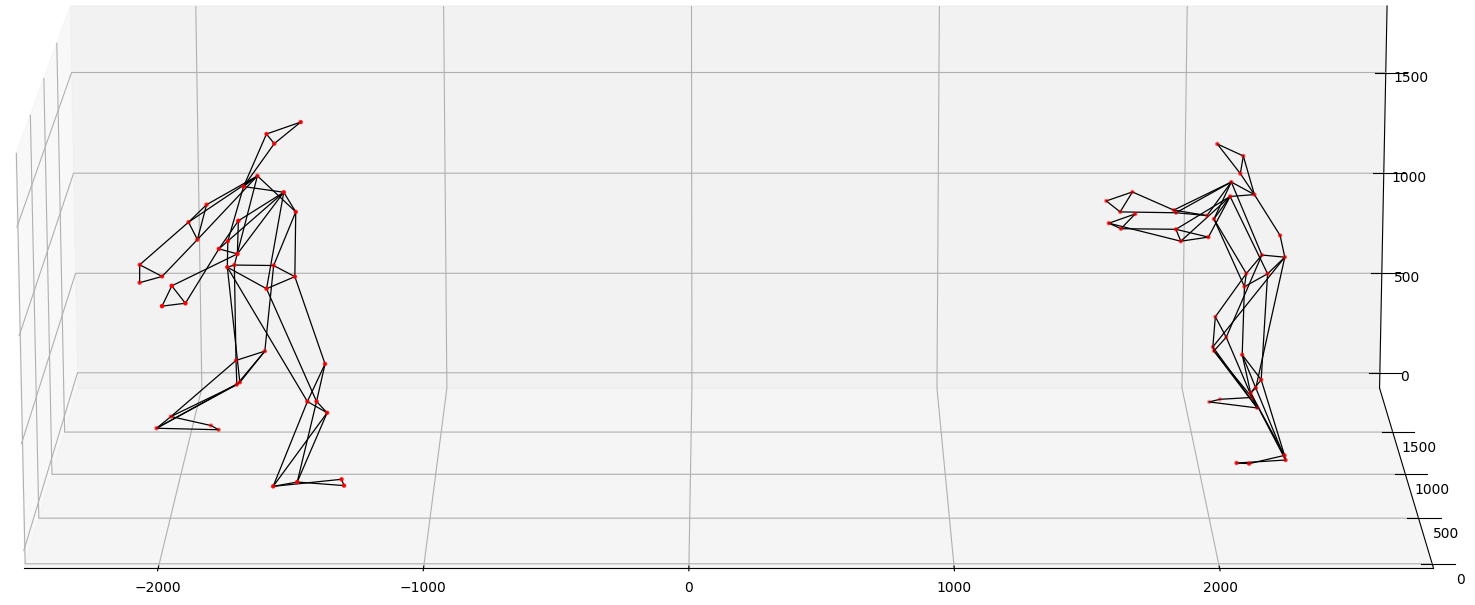
\includegraphics[width=0.75\textwidth]{bodyMarkersExampleMoCap.png}
    \caption{Video frame and MoCap scene with infrared cameras and markers}
    \label{fig:mocap_scene}
\end{figure}
\vspace{-1.5\baselineskip}
However, marker-based MoCap had limitations, including occlusion 
(when markers were hidden from view), inaccuracies, and the need for time-consuming calibration processes. 
These limitations led to the development of markerless MoCap technology. 
Markerless MoCap uses computer vision algorithms to track and reconstruct movement without the need for physical markers. 
This approach relies on complex algorithms that can identify and track features of the human body, 
such as joint positions and skeletal structure, from video footage.
%\begin{figure}[H]
%    \centering
%    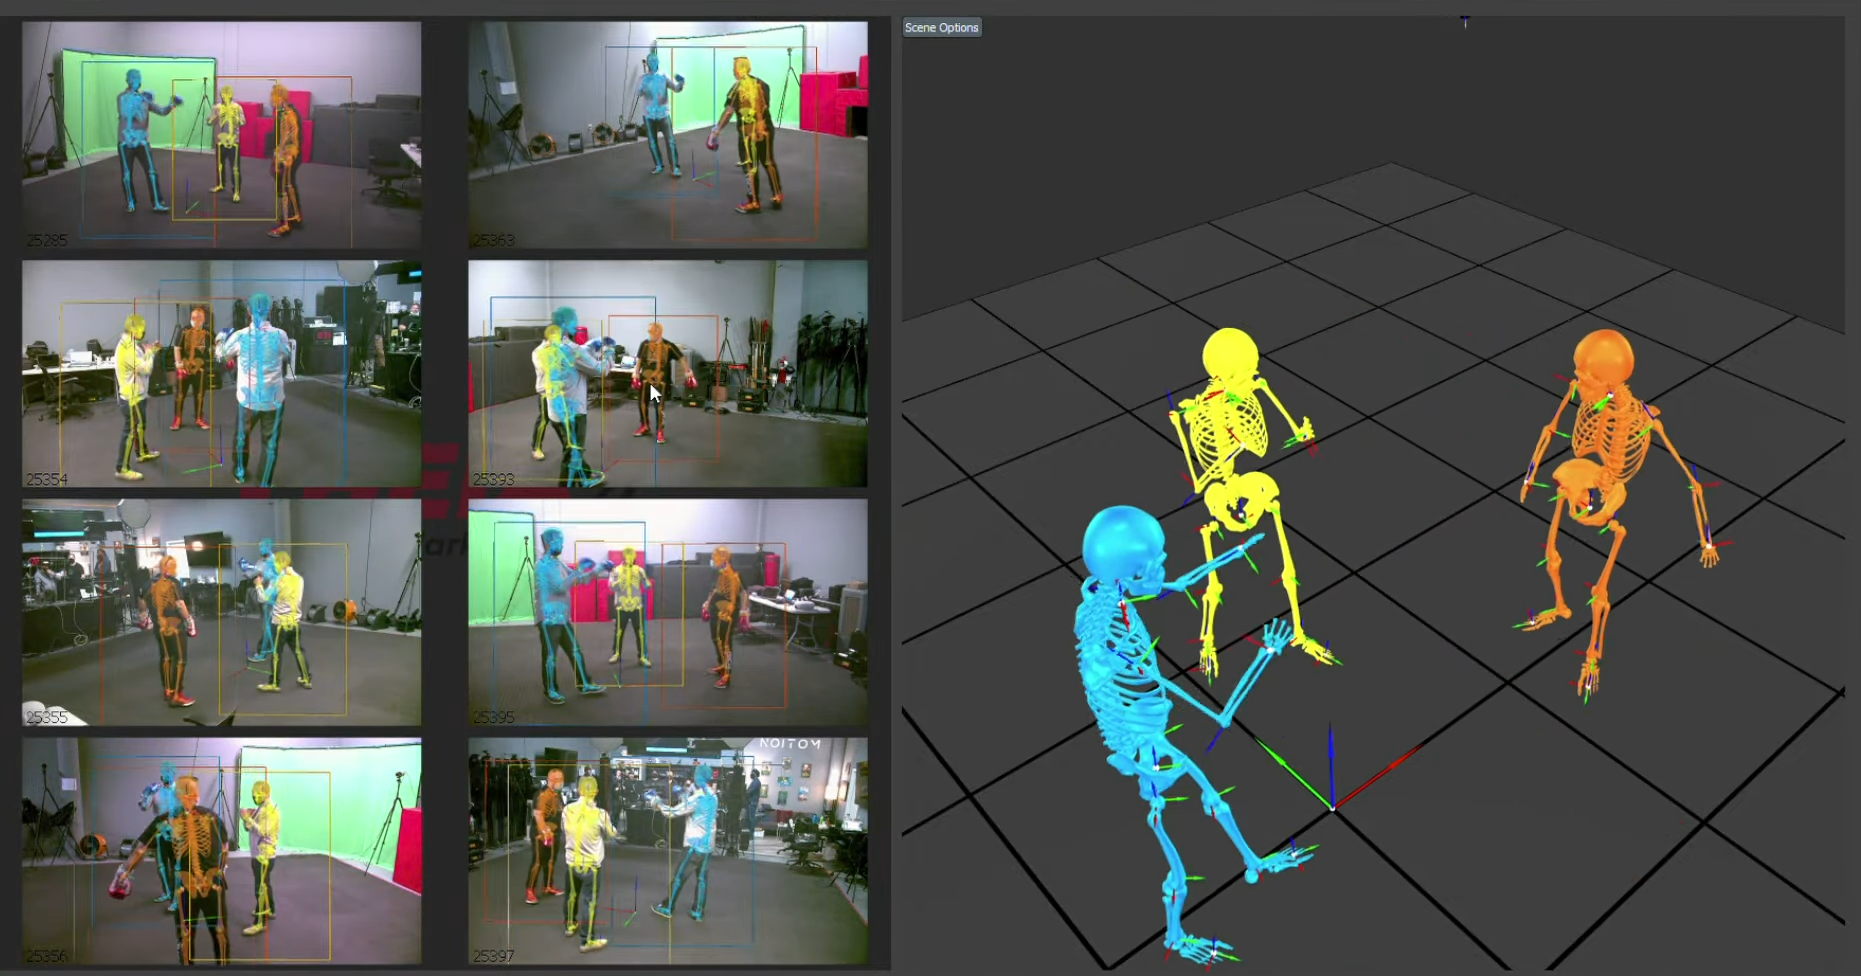
\includegraphics[width=0.7\textwidth]{MoCapMarkerlessQualisys.png}
%    \caption{Markerless MoCap scene}
%    \label{fig:mocap}
%\end{figure}

\section{Motivation}
While relationships between emotions and facial expressions or voice changes have been widely explored, 
leading to the availability of feasible methods for real-time automatic analysis, 
full-body movement has not been equally investigated. 
Various studies have shown great potential for inferring about emotions and many other human activities \cite{Bachmann:2020, preiler:2023}. 
Being able to automatically analyse the origin of movement could improve human performances, 
prevent injuries, promote physical activity, develop cognitive and motor rehabilitation strategies \cite{piana:2016}. 

For this reason, the research in human movement has branches in various fields of study such as biomechanics and neuroscience \cite{vaessen:2019}, 
experimental psychology, and theories from the arts and humanities \cite{camurri:2016}. 

The progress made in this field still does not allow a complete and robust classification of the origin of movement, in an automated way, 
because this relies mainly on arbitrary thresholds to distinguish between different origins and current state of the body, 
like if it is moving or standing still. 
For example, to recognize the instant when a movement starts it is required to manually tune 
minimum speed values that are difficult to automate and generalize for every context. 

Furthermore in movement recognition there are a lot of mid-level features, like the joint angles,
or the limb trajectories or the body segment coordination, which can be extracted and exploited by a comprehensive algorithm 
that weights every feature in an optimize manner, resulting in improved accuracy over all the possible approaches 
that work on them individually, because it could take into account the possible interactions and dependencies between them. 
An holistic approach in this way could leverage the complementary informations present in each feature by weighting them 
based on their relative importance. 
One last point to take into consideration is that algorithms based on single features could end up in overfitting the data
while the comprehensive one has more generalization capability. 

This research aims to contribute to the design of accurate and robust systems for the automated analysis of the origin of movement
by exploiting both the current techniques of analysis and the emerging ML approaches, 
which have become feasible thanks to advancements in computational capabilities of modern machines. 
